%
% Body text font is Palatino!
%

\documentclass[a5paper,pagesize,10pt,bibtotoc,pointlessnumbers,
normalheadings,DIV=9,twoside=false]{scrbook}

% twoside, openright
\KOMAoptions{DIV=last}

\usepackage{trajan}
 
\usepackage[ngerman]{babel}
\usepackage[utf8]{inputenc}
\usepackage[T1]{fontenc}

\usepackage[babel,german=guillemets]{csquotes}

\usepackage[sc]{mathpazo}
\linespread{1.05} 

\usepackage{verbatim} % for comments
\usepackage{listings} % for comments

%\setlength{\parindent}{10pt}
%\setlength{\parskip}{1.4ex plus 0.35ex minus 0.3ex}
%\setlength{\parskip}{1.4ex plus 0.35ex minus 0.3ex}

\usepackage{blindtext}
\newcommand{\q}[1]{>>\textit{#1}<<}

\usepackage{graphicx}

\title{Memory}   
\author{J.Y.} 
\date{\today} 

\begin{document}


%=========================================
\begin{titlepage}
		\centering{
			{\fontsize{40}{48}\selectfont 
			Memory}
		}\\
			
		\vspace{10mm}
		\centering{\Large{J.Y.}}\\
		\vspace{\fill}
		\centering \large{2021}
\end{titlepage}


%=========================================
\newpage{}
\thispagestyle {empty}

\vspace*{2cm}

\begin{center}
	\Large{\parbox{10cm}{
		\begin{raggedright}
		{\Large 
			\textit{Do what you think is interesting, 
			do something that you think is fun and worthwhile, 
			because otherwise you won’t do it well anyway.}
		}
	
		\vspace{.5cm}\hfill{---Brian W. Kernighan}
		\end{raggedright} 
	}
}
\end{center}

\newpage


%=========================================
%\blinddocument

\section{Memory Layout}
A typical memory representation of a C program consists of the following sections.
\begin{enumerate}
	\item Text segment
	\item Initialized data segment
	\item Uninitialized data segment
	\item Stack
	\item Heap
\end{enumerate}

\begin{figure}[!htb]
	\centering
	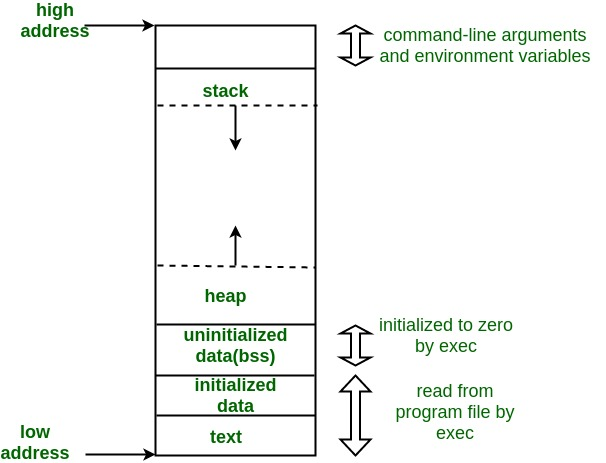
\includegraphics[width=\textwidth]{pictures/memoryLayoutC.jpg}
\end{figure}

\subsection{Text segment}
A \textbf{text segment}, also known as a \textbf{code segment} or simpley as \textbf{text},
is one of the sections of a program in an object file or in memory,
which contains executatble instructions.

As a memory region, a text segment may be place below the heap or stack 
in order to prevent heaps or stack overflows from overwriting it.

Usually, the text segment is sharable so that only a single copy needs to be 
in memory for frequently executed programs, such as text editors, the C compiler, 
the shells, and so on. Also the text segment is often read-only, to prevent program
from accidently modifying its instructions.


\subsection{Initialized Data Segment}
\textbf{Initialized data segment}, usually called simply the data segment. 
A data segment is a portion of the virtual address space of a program, 
which contains the global variables and static variables that are initialized by the programmer.

Note that, the data segment is not read only, since the values of the variables can be altered 
at run time.

This segment can be further classified into the initialized read-only and the initialized
read-write area.
For instance, the global string defined by char s[] = "Hello World" in C, and a C statement like 
int debug = 1 outside the main would be stored in the initialized read-write area.
And a global C statement like const char* str = "Hello World" makes the string literal "Hello World" 
to be stored in the initialized read-only area, and the pointer variable in the initialized 
read-write area.  

\subsection{Uninitialized Data Segment}


%=========================================
\begin{comment}
Just some notes, not visible in pdf.
\end{comment}


\end{document}

